
% title and thanks
\begin{titlepage}
\begin{center}

\textsc{\LARGE University of Manchester}\\[1.5cm]
\textsc{\Large School of Computer Science\\Project Report 2014}\\[0.5cm]

% Title
\HRule \\[0.4cm]
{ \huge \bfseries Using Machine Learning to predict personal expenditure \\[0.4cm] }
\question{I'm still not sure on the title, the report includes: prediction, historical finances and security}
\HRule \\[1.5cm]

% Author and supervisor
\begin{minipage}{0.4\textwidth}
\begin{flushleft} \large
\emph{Author:}\\
Pez \textsc{Cuckow}
\end{flushleft}
\end{minipage}
\begin{minipage}{0.4\textwidth}
\begin{flushright} \large
\emph{Supervisor:} \\
Dr Gavin \textsc{Brown}
\end{flushright}
\end{minipage}

\vfill

% Bottom of the page
%{\large \today}

\end{center}
\end{titlepage}
%TC:ignore
\begin{abstract}
A complete understanding of personal finances is becoming increasingly important as the average persons disposable income has decreased due to a changing financial climate.

The aim of this project is build to an application that makes it easier to manage a users personal finances. This is split into two halves, accessing historical information in an easy to understand way and using machine learning techniques to predict future financial information \todo{Still needs adjusting}. The security considerations of storing personal finance information is also considered.

This begins with a review of the existing commercial personal finance applications and the current techniques used to forecast time-boxed financial data, such as the value of a stock on the stock market, before detailing the design and implementation of the application.

Having completed the application, the performance the selected techniques are outlined, before discussing possible extensions to the application to improve it's accuracy and increase it's feature set and possible further research. \todo{This needs adjusting}
\\
\par\noindent{\textbf{Project Title}: Using Machine Learning to Predict Personal Expenditure \\
\textbf{Author}: Pez Cuckow \\
\textbf{Degree}: Computer Science with Business and Management \\
\textbf{Supervisor}: Dr Gavin Brown} \\

\par\noindent{\small{\bf Keywords:} Markov Chain Models, Weighted Arithmetic Mean, Responsive Web Design, Web System Security}

\end{abstract}
%TC:endignore

\clearpage
\vspace*{1.4in}
\begin{center}
  {\textbf{Acknowledgements}} \\
\end{center}
\begin{quotation}
  Thanks everyone, y'all great.
\end{quotation}

% define words
\newglossaryentry{transactor}
{
  name={transactor},
  description={somewhere money is spent, e.g. Tesco, Sainsbury's, Byte Cafe.}
}

\newglossaryentry{transaction}
{
  name={transaction},
  description={a single movement of money from/to a Transactor}
}

\newglossaryentry{category}
{
  name={category},
  description={transactors have a category and a subcategory, e.g. Tesco = Shopping, Groceries}
}

\newglossaryentry{reference}
{
  name={reference},
  description={the memo or message that is included on the bank statement with a transaction}
}

\newglossaryentry{mapping}
{
  name={mapping},
  description={this connects the reference found on a statement to a Transactor. e.g. Snbs, Sains => Sainsbury's}
}

\newglossaryentry{globaltransactor}
{
  name={global transactor},
  description={the system holds two collections of transactors and mapping's, the global ones
are shared between all users, and only accessed with the admin panel.}
}

\newglossaryentry{usertransactor}
{
  name={user transactor},
  description={unique to each user}
}

% start of document
\tableofcontents
\listoffigures
\listoftables
\printglossaries

\clearpage

% start of writing
\begin{comment}
This chapter puts the work into context. Having read it, the reader should be left in no doubt as to:

- the topic area to which the work applies
- why the work is being done
- what else has been done in the area and by whom
 - how the author proposes to tackle the problem: The project proposal is often expressed in terms of a main objective and possibly one or more additional objectives. It is useful to define "milestones" or "sub-goals" that mark the progress towards the objectives. 
 - It is common to end this chapter with a brief overview of each of the subsequent chapters of the report.
 
\end{comment}

\chapter{Introduction}
\label{cha:introduction}
Traditionally the management of personal finances is performed by viewing bank statements provided by the users bank. In the modern age of `Internet banking', banks offer a limited set of tools that mimic the paper statements seen historically.

This project sets out to build an online application that can be used to manage personal finances. There are two main parts of the project; firstly users can upload bank statements, which are displayed and navigated in an intuitive manner; secondly, once the application has enough historical data, predicting the users future outflow.

\section{Motivation}
There are four main steps when producing and using a budget: recording previous expenses, sorting these into categories, using this historical information to estimate future expenditure, and evaluating the accuracy of predictions based on the new information and adjusting accordingly.

Since the liquidity crisis of 2009 \parencite{gore2010}, budgets have been squeezed and the average personal disposable income has fallen significantly, hitting a nine-year low in 2012 \parencite{barnard2012households}. Experts suggest that ``Budgets are essential for financial planning'' \parencite{wsj2013budget}, research suggesting that personal budgets lead to a ``positive impact'' on ``mental wellbeing'' \parencite{tlap2013budget} and guides from UCAS, the UoM SU Advice Centre and The Manchester University Crucial Guide encouraging use of budgeting, it is clear that producing a budget is of benefit.

In an informal survey\footnote{Appendix \ref{app:budgetsurvey}} by the researchers, however, the majority of students questioned did not heed this advice, and were not following a budget. Producing an easier way to manage personal finances and predict future outflow can hopefully reduce the barriers to entry for creating budgets and increase the people using one.

Increasing use of debit cards \parencite{bbc2010debit} means that bank statements contain more and more information about where people spend their money. With access to those bank statements now provided online, and most UK banks offering the option to export \gls{transaction} history, individual users can collate a database of their personal spending habits.

The increasing availability of this data, combined with more detailed \gls{transaction} history makes it potentially possible to automate the four main steps of producing a budget, and this is the main objective of the project.

\section{Aims and Objectives}
%\plan{Things I set out to do, designed by talking to people to get an idea of features they would like}
The key objectives of this project can be split into three parts, the management of statements, making predictions of future outflow using those statements and ensuring a high level of security.

\subsection{Statement Management}
Implement an intuitive way to view and manage personal finances.
%
There are several key parts to this, upload and parsing of \glspl{transaction} from statements downloaded from the users bank, resolving the \glspl{reference} found on the statement to the real world business they represent and categorising the individual \glspl{transaction} to make them easier to understand.
    
\subsection{Prediction}
Accurately predicting a users future \glspl{transaction} based on their \glspl{transaction} history.
%
The prediction should be made using a model that is fitted to each users individual spending patterns, and is evaluated in order to improve the model.
%
The application will need to predict whether or not spending will occur and how much money will be spent.

\subsection{Security}
The project should be secure and uphold the high security expectations of users uploading their personal information.
%
The application will deal with information of a sensitive nature, therefore strong security techniques are of high importance to ensure no loss of personally identifiable information. 
% 
The project should take this into account, considering possible attack vectors and taking steps to mitigate those attacks.

\section{Overview of Report}
\plan{This report covers some of the key design decisions, implementation decisions and then what the application does}

Chapter \ref{cha:background} reviews existing commercial personal finance applications and existing techniques used to forcast time-boxed financial information.

Chapter \ref{cha:design} details the key design decisions made when planning the software and how the techniques in the background research are applied.

Chapter \ref{cha:implementation} includes implementation specifics of some of the features outlined in the design, focused particularly on features that were difficult to implement.

Chapter \ref{cha:results} gives an outlined of the finished applications features through the use of screenshots in a walkthrough.

Chapter \ref{cha:testing} reviews the performance of the application in terms of prediction accuracy and user experience. \todo{Does it?}

The report concludes in chapter \ref{cha:conclusions} which compares the project aims to what was achieved, suggests further enhancements that could be added to the application and outlines some further research areas.

\todo{This needs to be completed}
\chapter{Background}
\label{cha:background}

\begin{comment}
Chapter 2: Background and literature survey
This chapter should give essential background information with references to published material in research papers, books, URLs, magazine articles and even newspapers. Expand on any references to other work that have been mentioned in Chapter 1. Refer to the notes on references (below) for the preferred way of referencing publications. The reader, stimulated by the presentation of ideas in this section, may be led to consult some or all of the referenced publications. This section will be useful for any student in a subsequent year who wishes to take the project further.
\end{comment}

As outlined in Chapter \ref{cha:introduction} the project consists of two major parts: a financial management service, which can be used to view historical spending and gain understanding of personal finances; and a forecasting element which predicts how much spending will occur in the future. 
\question{Include this?} \question{Technically it's spending or receiving "transaction" but this becomes very wordy?}

\section{Statement Management}
There are existing applications that implement similar features to the money management aims of this project\question{Mention the current "bad" internet banking here?}, most notably Lloyds TSB Money Manager, the first and only personal money management application provided by a UK bank and Mint.com a United States (US) only personal finance service \parencite{lloyds2014moneymanager, mint2014whatismint}.

\subsection{Lloyds Money Manager}
The service is available to Lloyds TSB current account holders as part of their online banking and it's features revolve around documenting historical spending \parencite{lloyds2014money}.

The key features include:
\begin{itemize}
\item Categorising spending
\item Creating spending plans per category
%\item View dates money came in and out in a calendar
\item Viewing money spent per category
\item Track progress of budget targets
\end{itemize}

Customer reviews of the service highlight the usefulness of spending analysis screen, which includes a breakdown of spending in each \gls{category} (Fig. \ref{fig:moneymanager}, as well as the spending calendar, which displays money spent in a day by day format.
%
The reviews, however, also highlight some shortcomings, noting that changes to categories are not reflected immediately, categories are often incorrect and that it's not possible to override the \gls{category} for a single transaction, for example food bought at a petrol station is placed in the Car \gls{category} and cannot be moved \cite{moneywatch2011lloyds, moneysupermarket2011lloyds}.

\begin{figure}[h]
    \centering
    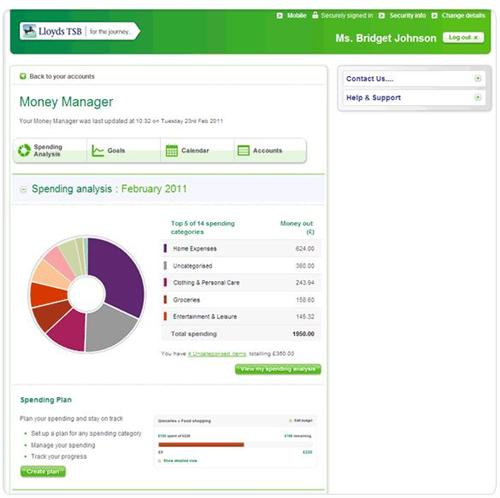
\includegraphics{background/moneymanagerchart}
    \caption{Spending Analysis by category on Money Manager \parencite{lloyds2014money}}
    \label{fig:moneymanager}
\end{figure}

A key advantage of the money manager is that Lloyds already have access to their customer data, so there is no data entry or upload required, which could be confusing and off-putting to potential users.

\subsection{Mint.com}
Mint.com offers very similar features to LLoyds but it limited to the US. However, Mint automatically logs into the users online bank account and downloads their statements authenticating with their banking username and password. It's reported that this feature relies on the use of application programming interface's (API) at each bank which Intuit (the company behind Mint) have negotiated access individually, though Intuit have published no information to support or dispute this \cite{stackoverflow2012bankingapi, stackoverflow2012bankingapi2}.
% 
Although this feature is clearly useful and saves time for the users, it does make Mint responsible for storing their customers Internet banking passwords and presumably involves fee payments to the banks providing these API's. \question{Should I have more detail on what mint/lloyds do?}
%
For these reasons it was decided that automatic statement uploading was outside of the budget and scope of this project, however, the project should support manual upload of statements to avoid date entry of users. \question{Does this need backing up?}

\subsection{Mobile Apps}
Mobile applications or `apps' as they are commonly known have seen a surge in popularity since the release of startphones and are a common target for small pieces of software, such as financial organisation \parencite{purcell2011half}.

The three most popular iPhone personal financial applications \cite{itunes2013topapps}, at the time of planning the project, all offered features very similar to those found in the Lloyds Money Manager and Mint. The most popular features being grouping money by \gls{category} and graphs of spending history.
% 
However, they all had the same drawback, the user had to manually enter all of their transactions and set categories for them, which appears time consuming and error prone, particularly on a mobile app \cite{spendee2014spendee,budgt2013budgt,bluetags2014pocket}.

The increase of mobile usage should be considered when planning the features of the project, with the project ensuring mobile compatibility and if possible, avoiding manual data entry. \plan{This needs improving}

\section{Prediction}
%\plan{Ways other people try to predict the future expenditure (in stocks etc...)}

There are various approaches to making predictions of financial spending, each with their own advantages and disadvantages \question{Not sure if this is relevant}. Predicting future transactions before they occur is technically similar to the work done by investors on the stock market, where the objective is to predict whether the value of a stock will fall or increase in order to make buy/sell decisions.

Preifer and Carraway demonstrated that Markov Chain Models can be used to model customer relationships with a business and predict the expected value of a marketing engagement with an individual customer. By creating a transition matrix of a particular customer transitioning from not spending to spending and visa versa over five periods\footnote{An `illustration' assuming a customer will never return after 5 months of not spending}, they were able to estimate the likely-hood of a spend occurring in a given period, Fig. \ref{fig:preifermarkovchain} shows a graphical representation of the model that was produced, the states represent the five periods, where $p_{i}$ is the probability of the transition occurring during period $i$ \cite{pfeifer2000modeling}.
% 
The paper is able to calculate the expected loan to value ratio (LTV) for the customer over the periods, by taking a matrix costs and gains associated with a purchase in each period and multiplying that by the probability of a purchase occurring taken from the transition matrix. This gives the expected present value for each period, which can be used to decide when to end a relationship with a customer (preventing the costs).
%
They demonstrate applying Markov Chain Models to a larger dataset, calculating the optimal policy for ending relationships with customers depending on varying costs concluding that the use of MCM's is an effective way of making customer relationship decisions. However, this paper assumes the company performing these predictions already knows how much money a customer will spent during each interactions and is focussed around calculating the probability of a spend occurring. An implementation applied to the personal spending space will require a way to predict the value of the future transaction.
\question{Mention what HMM's are here?}

\begin{figure}[h]
    \centering
    %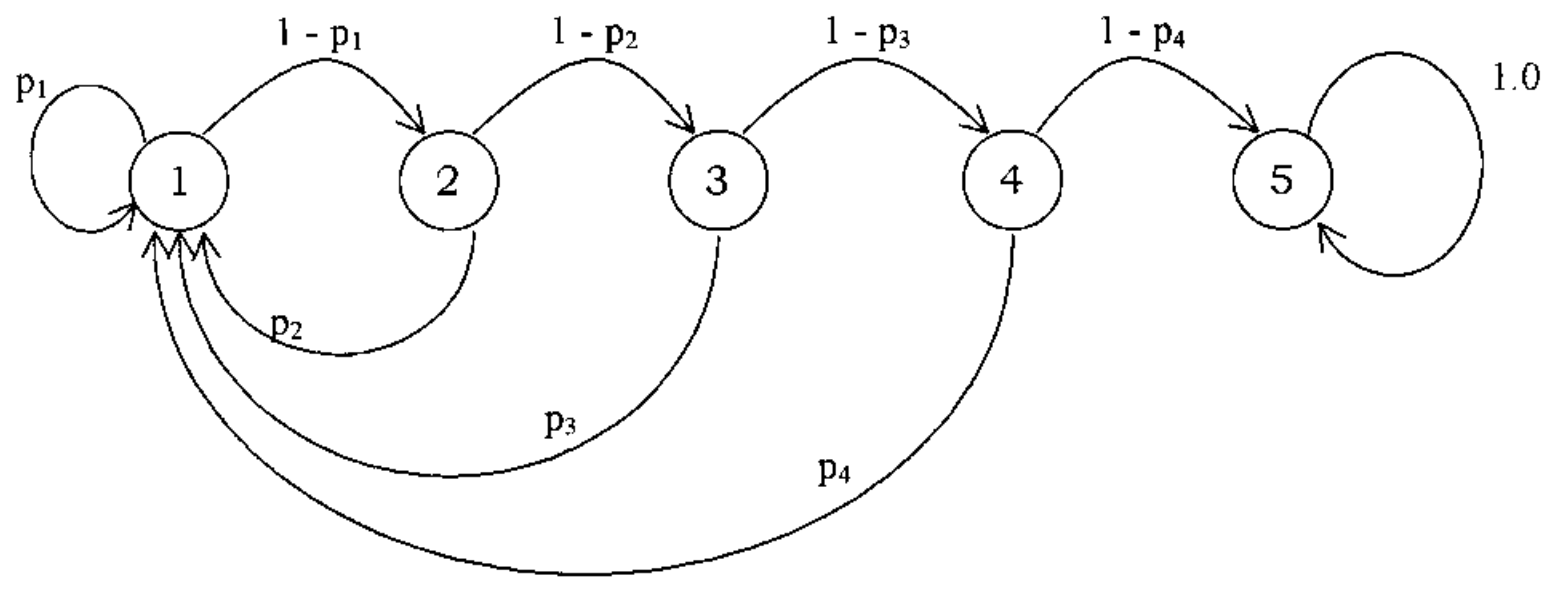
\includegraphics[width=\textwidth]{background/markovchain}
    \begin{tikzpicture}[start chain=going right]
    \node[state, on chain]                 (1) {1};
    \node[state, on chain]                 (2) {2};
    \node[state, on chain]                 (3) {3};
    \node[state, on chain]                 (4) {4};
    \node[state, on chain]                 (5) {5};
    \
    \draw[
        >=latex,
    %   every node/.style={above,midway},% either
        auto=right,                      % or
        loop above/.style={out=75,in=105,loop},
        every loop,
        ]
     (1) 	edge[bend left] node [above]{$1 - p_{1}$}   (2)
      		edge[out=145,in=220,loop,looseness=6]             node {$p_{1}$}   (1)
     (2) 	edge[bend left] node[above]{$1 - p_{2}$}   (3)
      		edge[bend left=90,,in=120]             node {$p_{2}$}   (1)
     (3) 	edge[bend left] node[above] {$1 - p_{2}$}   (4)
     		edge[bend left=90,in=105,]             node {$p_{3}$}   (1)
     (4) 	edge[bend left] node [above]{$1 - p_{2}$}   (5)
     		edge[bend left=90,in=90]             node {$p_{4}$}   (1)
     (5) 	edge[out=40, in=320,loop,looseness=6] node[right]{$1.0$}   (5);
    
    
    % The \draw path is like the one above.
    \end{tikzpicture}
    \caption[Markov Chain Model of customer spending]{Markov Chain Model for a particular customer over five periods \parencite[Adapted from Fig. 1]{pfeifer2000modeling}}
    \label{fig:preifermarkovchain}
\end{figure}

% OTHER PREDICTION
Research by Singh et al., from the Massachusetts Institute of Technology, studied the spending behaviour of 52 adults and investigated the impact of social interactions, including text messages, phone calls and face-to-face meetings, on the participants spending in order to predict their spending behaviour. Using a Na\"{i}ve Bayes classifier and selecting a subset of their available features using an Information Gain approach, choosing those with most relevance to each classification task, they were able to correctly classify whether the participant would overspend, explore a diverse range of businesses and remain loyal to a business with 72\% overall accuracy. They concluded that social factors, were better ``predictors of spending behaviour'' than personality traits, which had been previously studied \parencite{singh2013spendingbehaviour}.
%
Although this paper did not study the affects of the participants previous transactions on spending, they were able to predict the users spending behaviour, highlighting that factors other than the transaction history may be of importance when trying to predict a users future outflow. However, the paper does not attempt to make a prediction of the amount spent or how many transactions occur.

% AVERAGES
Smoothing is typically applied to financial market data, for example the value of a particular stock on the FTSE 100. The most common techniques are simple, weighted and exponential moving averages, which all reduce the noise found in the data potentially revealing an orderly process, by removing outliers found in the data. The result of this effect can be seen in Fig \ref{fig:dashweightedaverages} \parencite{dash2012movingaverages}.

\begin{figure}[h]
    \centering
    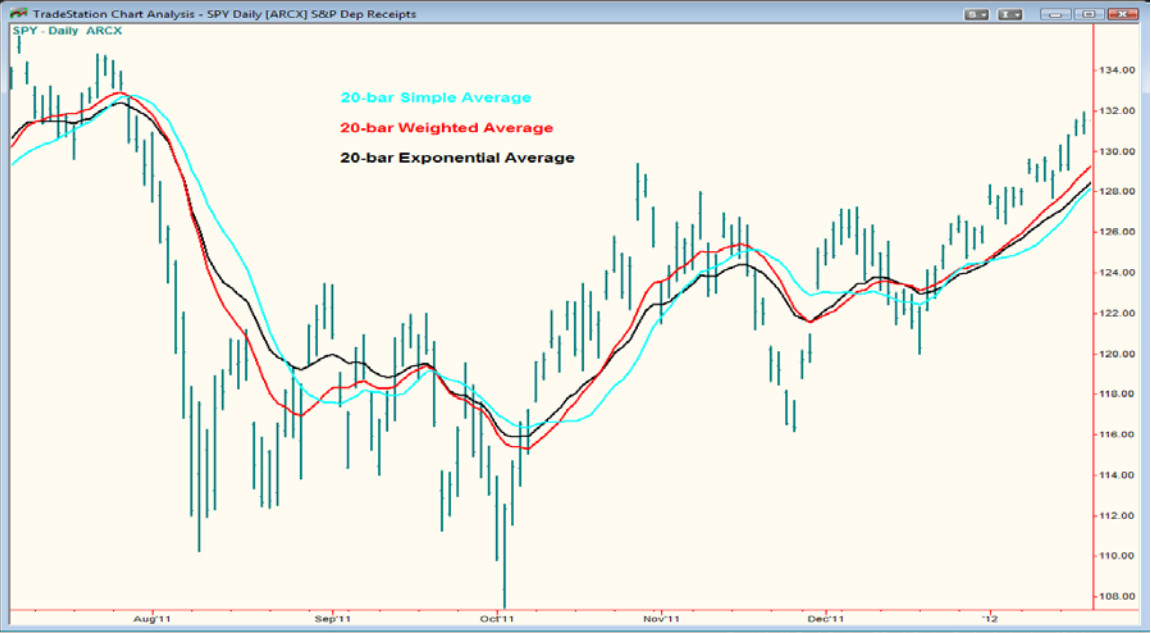
\includegraphics[width=\textwidth]{background/movingaverages}
    \caption[SMA, WMA and EMA of the S\&P500]{Simple Moving Average (MA) [blue], Weighted MA [red] and Exponential MA [black] of the S\&P500 \protect\footnotemark \parencite[Fig. 5]{dash2012movingaverages}}
    \label{fig:dashweightedaverages}
\end{figure}
\footnotetext{A stock market index of 500 American companies, the US equivalent of the FTSE 500}

These techniques can be applied to a discrete set of numerical time series data, such as personal expenditure over time in order to make an estimate of what the next value in the series will be \parencite{filliben2003nist}. A prediction can be made using the formula in Fig. \ref{fig:weightedmeanforumla}, where $w_{i}$ is the weight and $x_i$ is the value at time period $i$. Simple smoothing is the equivalent of $w_i = 1$, while exponential smoothing is based around a negative exponential law such as $w_i = e^{-n+i}$, both are examples of weighted smoothing and the weights can be decided in different ways depending on what is being predicted. Time periods with a higher weight have a greater affect on the mean, so in order to make a future prediction, the most recent time period would have a higher weight. \question{The chosen implementation details in the design section}

\begin{figure}[h]
    \centering
    \[
        \frac{w_1 x_1 + w_2 x_2 + \cdots + w_n x_n}{w_1 + w_2 + \cdots + w_n}.
    \]
    \caption{Using weighted smoothing to predict a future value}
    \label{fig:weightedmeanforumla}
\end{figure}

% Holt winters extends smoothing, to take into account trends in data
Smoothing (and therefore prediction) can be extended to take into account trends and possible seasonal fluctuations using double and triple smoothing, respectively. A technique known as `Holt-Winters double exponential smoothing` takes into account trends in data, which single smoothing does perform accurately with, by factoring the weighted average growth between previous the time series when calculating the average for each period \parencite{kalekar2004holtwinters}. \question{A demonstration of this is in chapter X?}
% 
Extending the calculation into double and triple smoothing when estimating a users future outflow was decided as a possible extension for the project. \question{Where to mention this?} 

\section{Security}
\question{Should I mention the password entropy paper here? Currently in design}



\include{chapters/chapter3}
\include{chapters/chapter4}
\include{chapters/chapter5}
\include{chapters/chapter6}
\include{chapters/chapter7}

%% References
% There are a number of schemes for presenting references to the reader. Most publications are very strict about their presentation and, unfortunately, there is no unanimity of format across the range of relevant publications. The recommended method, used in IET and IEEE journals, is to identify each reference with a number located at the appropriate point of the text in square brackets, e.g. [42]. This is the recommended format for project reports in Computer Science. The list of references included in your report must give all the relevant information to enable the reader to find it.

% references
\printbibliography

% appendix
\begin{appendices}

\chapter{Survey} \label{app:budgetsurvey}
Informal survey of 12 CS students in the third year lab. 

Questions:
\begin{enumerate}
\item Do you currently make a budget?
\item Do you stick to that budget?
\item Do you find your budget has a `positive' impact?
\end{enumerate}

% Booktabs require to add  to your document preamble
\begin{table}[h]
\centering
\caption{Survey Results}
\begin{tabular}{@{}llll@{}}
\toprule
       & \multicolumn{3}{l}{Question} \\ 
Answer & 1.       & 2.      & 3.      \\ \midrule
yes    & 5        & 1       & 3       \\
no     & 7        & 4       & 4       \\
n/a    & 0        & 7       & 5       \\ \bottomrule
\end{tabular}
\end{table}

\begin{comment}
Appendix A, B, C, etc.
These appendices can be very useful for giving detail that would otherwise disrupt the flow and readability of the report. They are given titles (e.g. "Appendix A: Example of the operation of the system") and bound in with the report. In general they are optional though, by convention, for a programming project, Appendix A often contains a non-trivial illustrative example of an input to the system and the corresponding output. For some projects, appendices may include tables of data. However, very long tables of data (more than about 10 pages) should be relegated to the Auxiliary Material, and not submitted as part of the Final Report. Program listings (apart from short code snippets) should likewise not be submitted as part of the Final Report.
\end{comment}

\chapter{Hashing Test} \label{app:hashingtest}

Implemented in PHP, test was run on a 2.7 Ghz Intel Core i7 with 16Gb of 1600Mhz DDR3 RAM.

\lstinputlisting[style=phpcolor]{code/passwordHashingTest.php}

\chapter{PHP Code} \todo{Needs a better name}

\begin{figure}
\lstinputlisting[style=phpcolor]{code/setTransactorMethod.php}
\caption{PHP Transaction->setTransactor(\$name) method source code}
\label{fig:settransactor}
\end{figure}

\begin{figure}
\lstset{style=phpcolor}
\begin{lstlisting}
if($dmy && $mdy || !$dmy && !$mdy)
    // ... prompt the user
else
    // ... continue conversion using the detected month format
\end{lstlisting}
\caption{Whether or not to prompt the user following month format detection}
\end{figure}
\chapter{Suggestion Wizard JSON}

The suggestion wizard is powered by AJAX, which makes JSON requests to a RESTful API on the backend, Fig. \ref{fig:json-examples} outlines an example set of communication.

\begin{figure}
    \begin{subfigure}[a]{\textwidth}
        \lstinputlisting[language=json]{code/suggestions.json}
        \caption{GET request sent \lstinline{/ajax/transactor/suggestions}}
    \end{subfigure}
    
    \begin{subfigure}[b]{\textwidth}
        \lstinputlisting[language=json]{code/map.json}
        \caption{POST request sent to \lstinline{/ajax/transactor/map}}
    \end{subfigure}
\end{figure}

\begin{figure}
    \ContinuedFloat   
    \begin{subfigure}[c]{\textwidth}
        \lstinputlisting[language=json]{code/create.json}
        \caption{POST request sent to \lstinline{/ajax/transactor/create}}
    \end{subfigure}
    
    \begin{subfigure}[d]{\textwidth}
        \lstinputlisting[language=json]{code/reply.json}
        \caption{Response from API following a successful map or create}
    \end{subfigure}    

    \caption{JSON encoded requests to the RESTful API}
    \label{fig:json-examples}
\end{figure}

\end{appendices}
